\documentclass[a4wide]{report}

\usepackage{amsmath}
\usepackage[a4paper, total={7in, 10.2in}]{geometry}
\usepackage{graphicx}
\usepackage[portuguese]{babel}
\usepackage[utf8]{inputenc}


\begin{document}

\noindent
{\bf Rafael V. Cacilhas  - Relatório 11 (\today)}

\vspace{0.5cm}

\section*{Exercício 1}

\subsection*{a) }
Queremos demonstrar que $\Delta E = E^{\alpha'} - E^{\alpha} = \sum\limits_{j = 1}^{N} u(r^{\alpha'}_{nj}) - u(r^{\alpha}_{nj})$. Para tal, usaremos o fato de que $u^{\alpha}_{ij} =u^{\alpha'}_{ij} $ para todo i,j diferente de n e separaremos a soma de n das demais:

\begin{equation*}
\Delta E  =\frac{1}{2} \sum\limits_{i = 1}^{N}\sum\limits_{j \ne i}^{N} \left( u(r^{\alpha'}_{i,j}) - u(r^{\alpha}_{i,j} ) \right)
\end{equation*} 

\begin{equation*}
\Delta E  =\frac{1}{2} \left( \sum\limits_{i \neq n}\sum\limits_{j \neq n,i}\left( u(r^{\alpha'}_{i,j}) - u(r^{\alpha}_{i,j} ) \right) + \sum\limits_{j \neq n} \left( u(r^{\alpha'}_{n,j}) - u(r^{\alpha}_{n,j} ) \right) + \sum\limits_{i \neq n}\left( u(r^{\alpha'}_{i,n}) - u(r^{\alpha}_{i,n} ) \right)\right)
\end{equation*} 

\begin{equation*}
\Delta E  =\frac{1}{2} \left( \sum\limits_{i \neq n}\sum\limits_{j \neq n,i}\left( u(r^{\alpha'}_{i,j}) - u(r^{\alpha}_{i,j} ) \right) + \sum\limits_{j \neq n} \left( u(r^{\alpha'}_{n,j}) - u(r^{\alpha}_{n,j} ) \right) + \sum\limits_{i \neq n}\left( u(r^{\alpha'}_{i,n}) - u(r^{\alpha}_{i,n} ) \right)\right)
\end{equation*} 

O primeiro termo, como discutido acima, é zero. Já o segundo e terceiro termo são iguais, pois apenas a ordem da soma é alterada. Assim:

\begin{equation*}
\Delta E  =\frac{1}{2} \left( 2\sum\limits_{j \neq n}\left( u(r^{\alpha'}_{j,n}) - u(r^{\alpha}_{j,n} ) \right)\right)
\end{equation*} 
\begin{equation}
\Delta E  =\sum\limits_{j \neq n} u(r^{\alpha'}_{j,n}) - u(r^{\alpha}_{j,n} )
\end{equation} 

No programa me.f90 a energia foi calculada da maneira local, deduzida acima, e da maneira global. As duas maneiras podem ser vistas descomentando as subrotinas relevantes e os resultados são idênticos.

\subsection*{b) }

Feito no programa me.f90.

\subsection*{c) }
Na Figura \ref{1c} vemos a energia em função dos passos de Monte Carlo para T = 30K.
\begin{figure}[!htb]
\centering
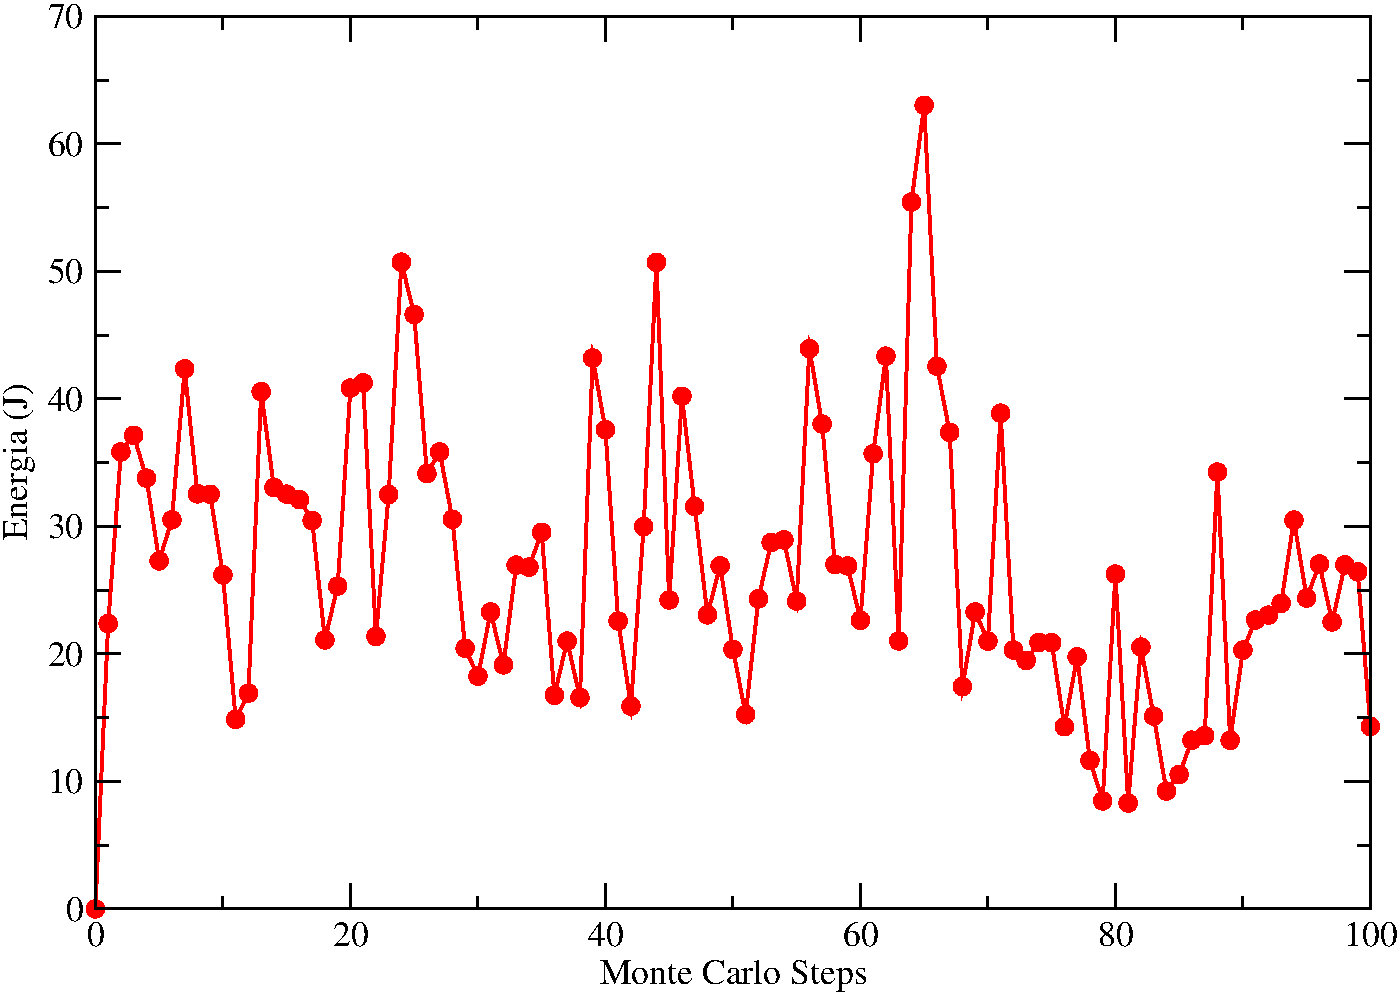
\includegraphics[width=0.32\textwidth]{saida.pdf}
\caption{Distribuição de energia em função dos passos de Monte Carlo.}
\label{1c}
\end{figure}

De modo a testar se o programa correlacao.f90 está calculando tudo corretamente utilizamos a sequência de números aleatórios $random\_seq.dat$ da última lista. O C(i) calculado está na figura \ref{2c}. Como pode ser visto, tudo parece estar em ordem, visto que temos um C(i) que começa em 1 e cai rapidamente para zero, como esperado.

\begin{figure}[!htb]
\centering
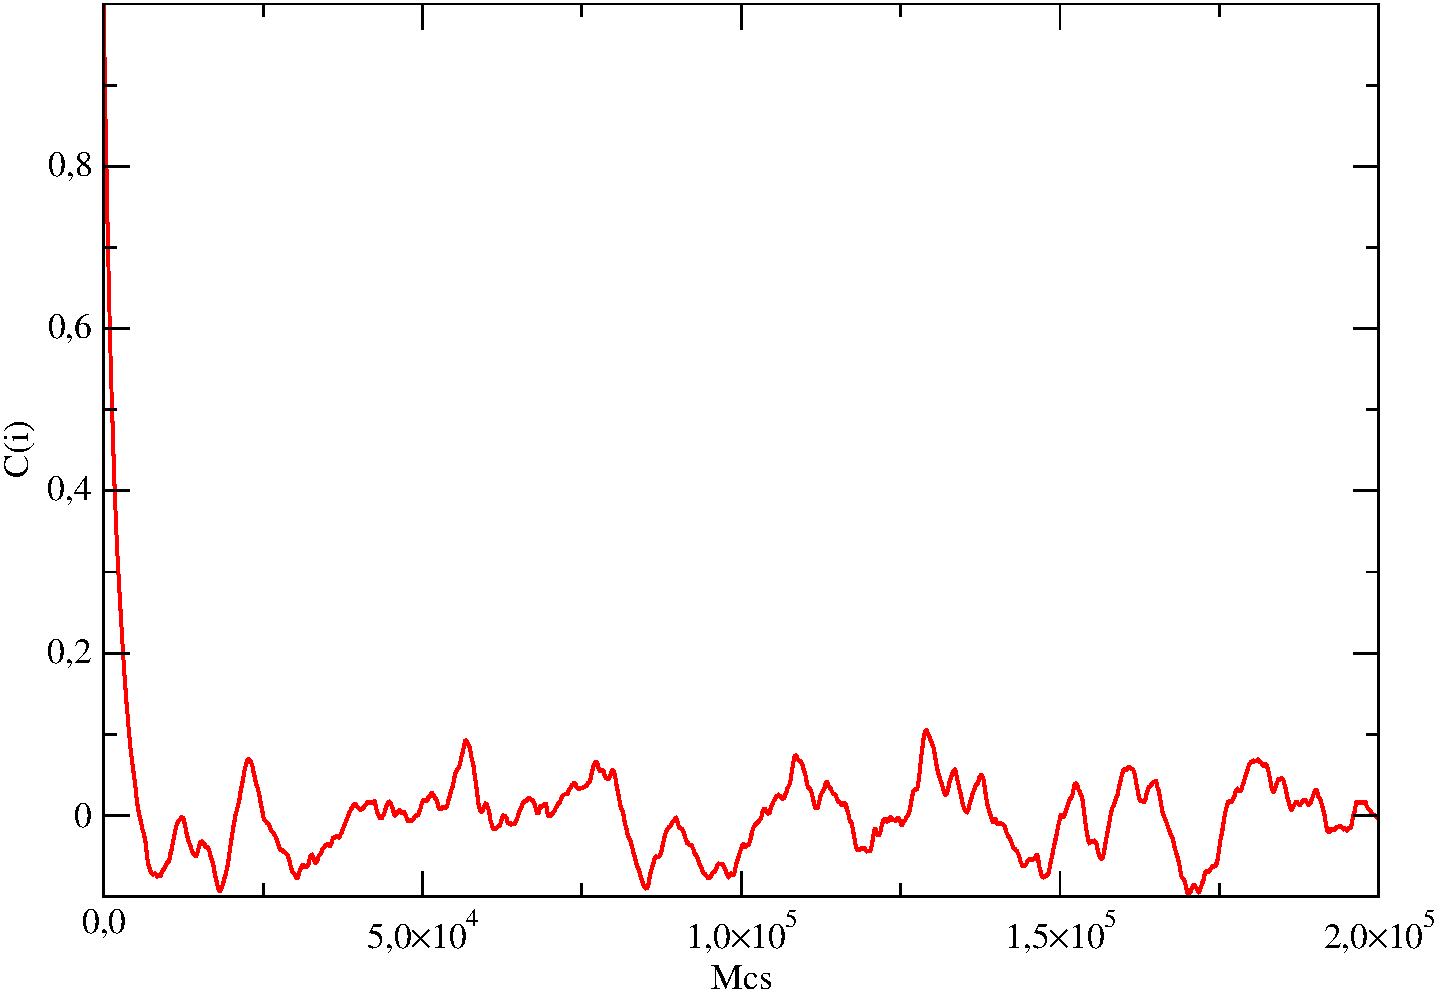
\includegraphics[width=0.32\textwidth]{teste.pdf}
\caption{Distribuição de energia em função dos passos de Monte Carlo.}
\label{2c}
\end{figure}


Ao calcular o tempo de auto-correlação integrado 2$\tau$ foi encontrado um problema visto que alguns valores são negativos e a interpretação disto não foi encontrada. Portanto a análise da correlação em função de $d_{max}$ foi feita utilizando diretamente o gráfico de C(i) visto na Figura \ref{3c}.


\begin{figure}[!htb]
\centering
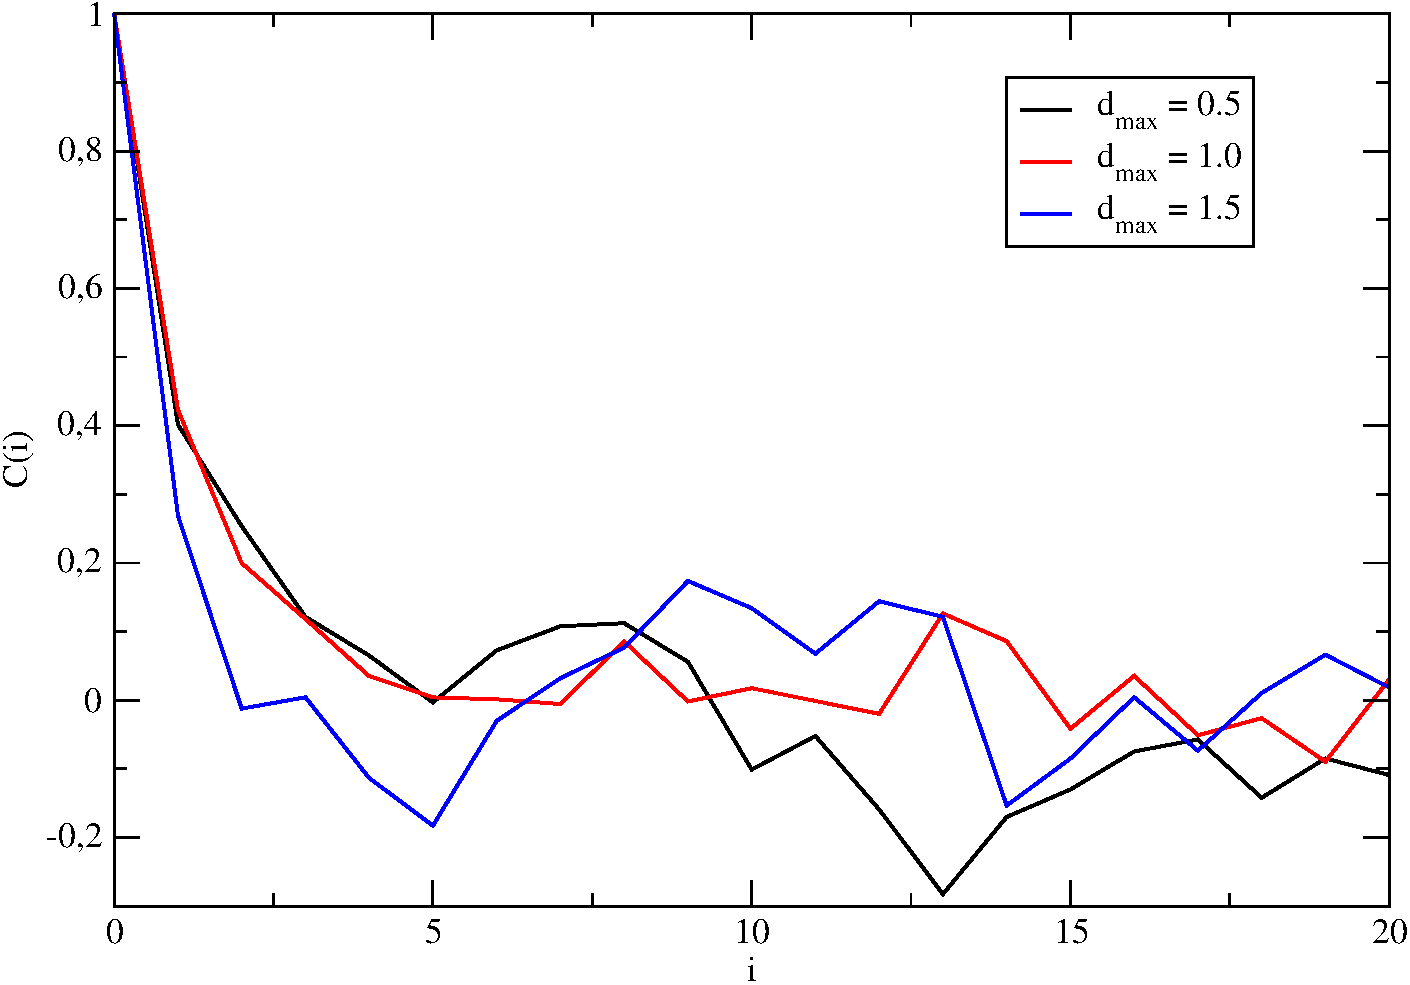
\includegraphics[width=0.32\textwidth]{ci.pdf}
\caption{C(i) para três valores de $d_{max}$.}
\label{3c}
\end{figure}

Como pode ser visto, para todos os valores de $d_{max}$ temos o comportamento esperado, onde C(i) começa em 1 e oscila em torno de zero. No entanto é visível que para $d_{max} = 1.5$ o valor de C(i) vai para zero mais rapidamente do que os demais. Assim sendo, este valor de $d_{max}$ produz as energias mais descorrelacionadas e seria a escolha adequada.


\subsection*{d)}
A energia média por partícula e o calor específico em função da temperatura pode ser visto na Figura \ref{1d}.

\begin{figure}[!htb]
\centering
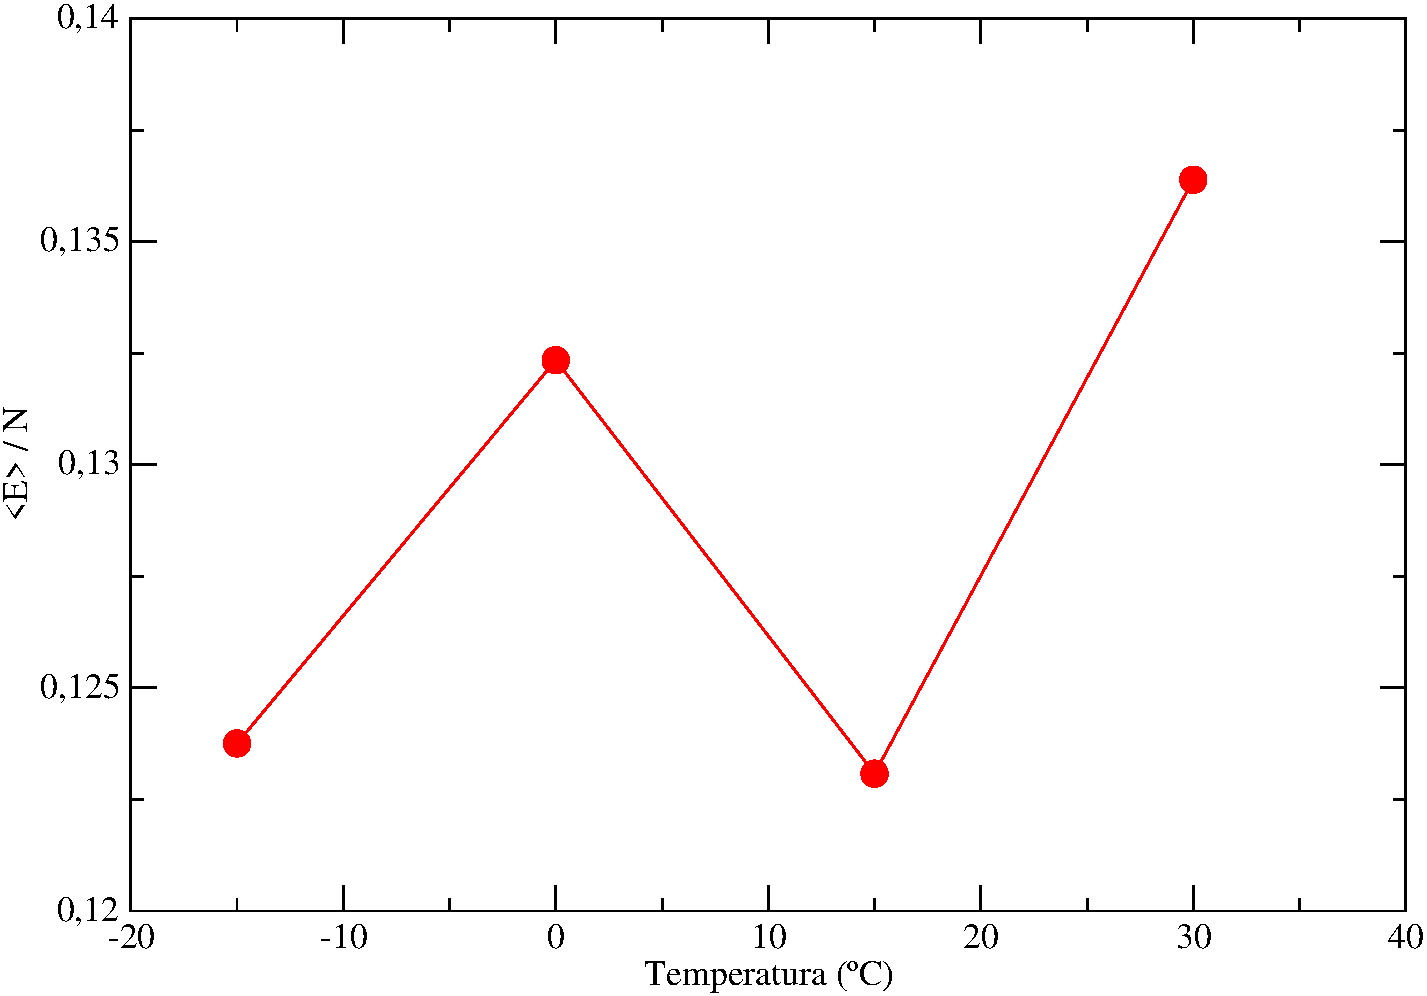
\includegraphics[width=0.32\textwidth]{energia.pdf}
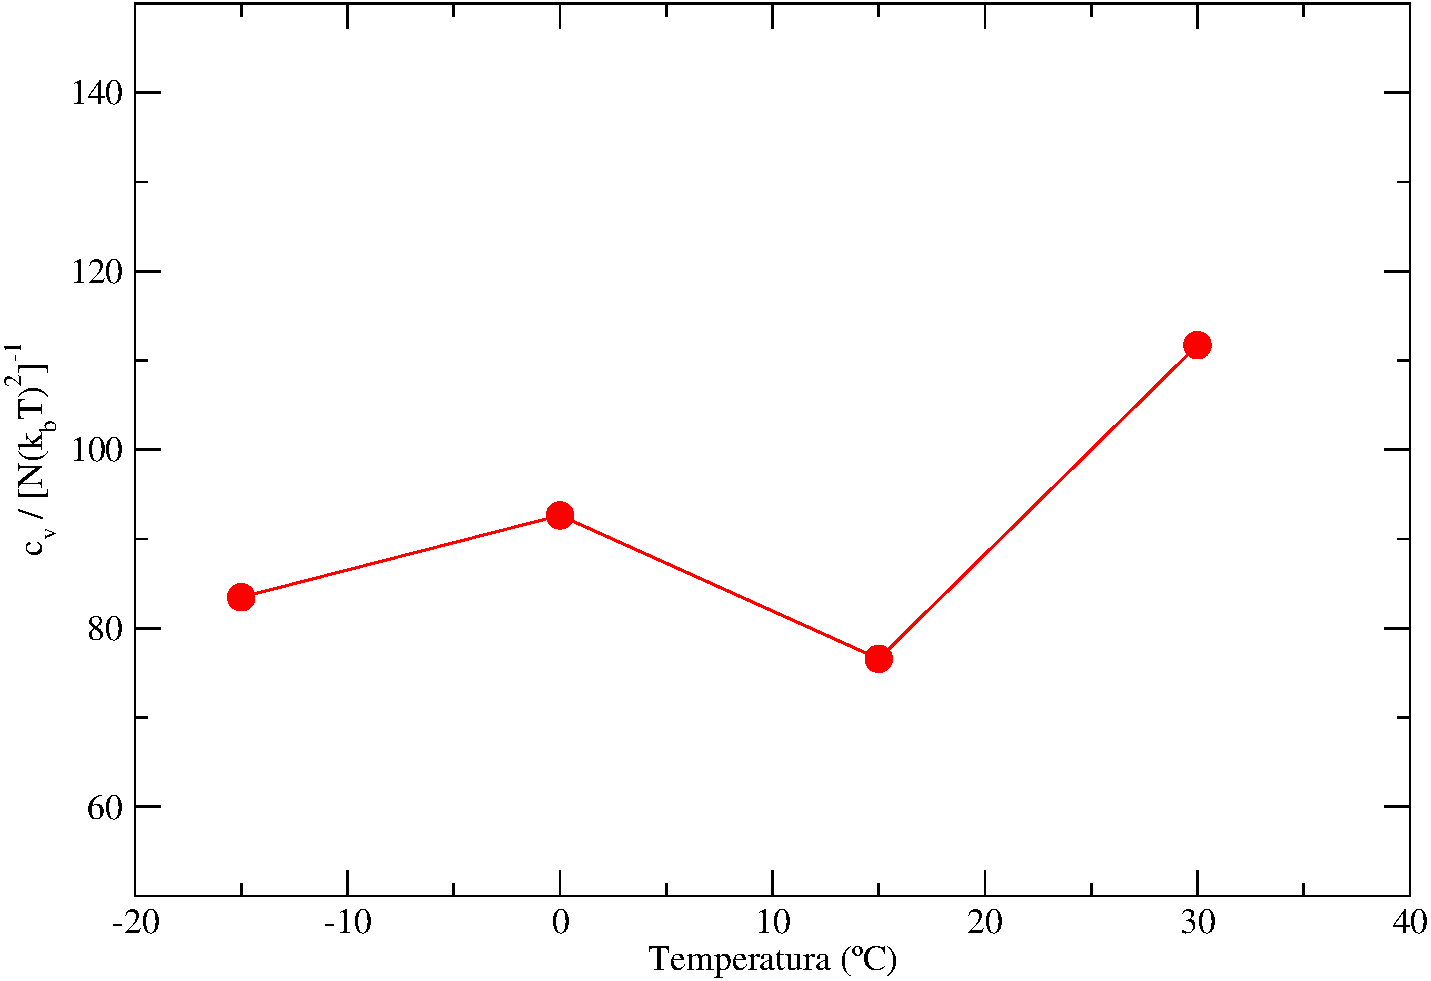
\includegraphics[width=0.32\textwidth]{cv.pdf}
\caption{Energia média por partícula (esquerda) e calor específico (direita) em função da temperatura.}
\label{1d}
\end{figure}

O histograma pode ser visto na Figura \ref{2d}.
\begin{figure}[!htb]
\centering
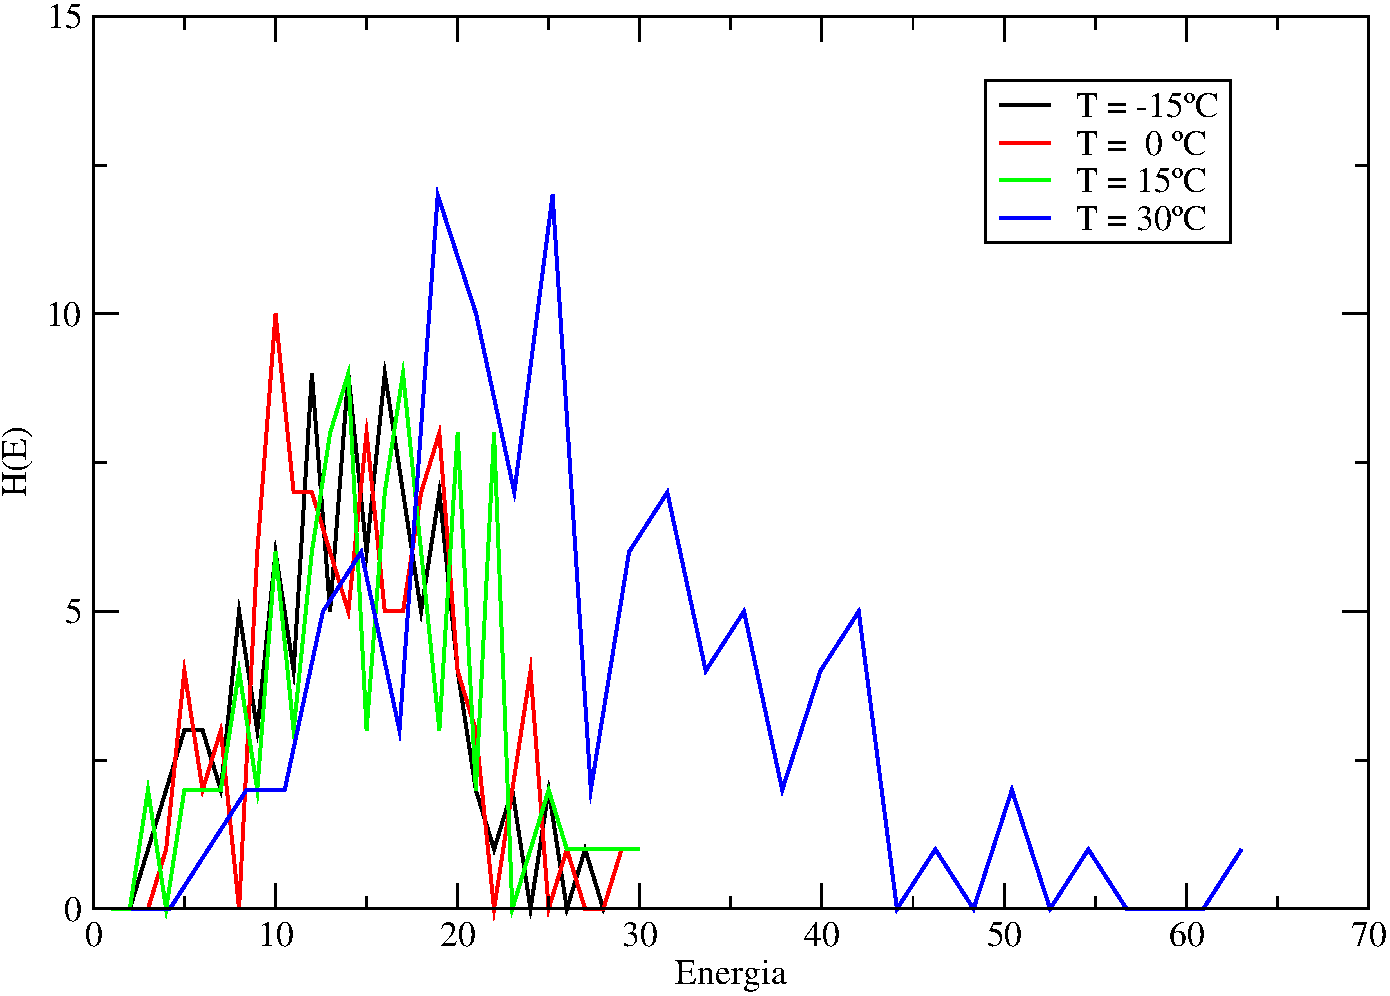
\includegraphics[width=0.32\textwidth]{hist30.pdf}
\caption{Histograma das energias em função da temperatura.}
\label{2d}
\end{figure}

\end{document}